% Pre-review integrity check (citations and reported numbers) of the draft manuscript in ../../manuscript.
% Build: pdflatex integrity_check.tex (twice). Chart: python3 fig_counts.py (writes fig_counts.pdf beside this file).
\documentclass[10pt,a4paper]{article}
\usepackage[margin=18mm]{geometry}
\usepackage[T1]{fontenc}
\usepackage[utf8]{inputenc}
\usepackage{textcomp}
\usepackage{lmodern}
\usepackage{booktabs,longtable,array,graphicx,xcolor,amsmath,tikz}
\usepackage[hidelinks]{hyperref}
\usetikzlibrary{arrows.meta,positioning}
\setlength{\parindent}{0pt}
\sloppy
\setlength{\emergencystretch}{3em}
\setlength{\parskip}{4pt}
\renewcommand{\arraystretch}{1.15}
\newcolumntype{P}[1]{>{\raggedright\arraybackslash}p{#1}}
\newcommand*{\BR}{\mathit{BR}}
\newcommand*{\Reth}{\mathit{Re}_\theta}
\newcommand*{\ReD}{\mathit{Re}_D}
\newcommand*{\Tu}{\mathit{Tu}}
\newcommand*{\Leff}{L_{\mathrm{eff}}}
\newcommand*{\etab}{\bar\eta}
\newcommand*{\deta}{\Delta_{\mathrm{mesh}}/\eta_{K,193}}
\renewcommand{\cite}[1]{[\texttt{#1}]}
\newcommand{\vS}{\textsf{S}}
\newcommand{\vNS}{\textbf{\textsf{NS}}}
\newcommand{\vSNS}{\textsf{SNS}}
\newcommand{\vM}{\textsf{M}}
\newcommand{\vR}{\textsf{R}}
\newcommand{\vMM}{\textbf{\textsf{MM}}}
\newcommand{\vNSF}{\textsf{NSF}}
\newcommand{\vNC}{\textsf{NC}}

\title{Pre-review integrity check of \texttt{main\_claude.tex}\\[2pt]\large citations and reported numbers}
\author{GT2027 draft, shaped film-cooling hole; check run 27 November 2026}
\date{}

\begin{document}
\maketitle
\vspace{-8mm}

\section*{Summary}

\textbf{Overall verdict: PASS WITH FINDINGS.} Every citation key resolves and every cited reference exists. Six
citation statements and six reported numbers disagree with their sources; ten numbers have no source in the files
checked. All are correctable without new computation, except where marked.

\begin{center}
\begin{tabular}{@{}l r r r r r r@{}}
\toprule
Population & checked & match & rounding & mismatch & no source & not checkable \\
\midrule
A1 cite keys resolve (53 keys) & 53 & 53 & -- & 0 & 0 & -- \\
A2 bib entries complete (53 entries) & 53 & 37 & -- & 16 gaps & -- & -- \\
A3 attributed claims & 69 & 48 & -- & 6 & 15$^a$ & 0 \\
B reported numbers & 191 & 165 & 5 & 6 & 10 & 5 \\
\bottomrule
\end{tabular}\\[2pt]
{\footnotesize $^a$ source not stored; no verdict given from memory.}
\end{center}

\begin{center}
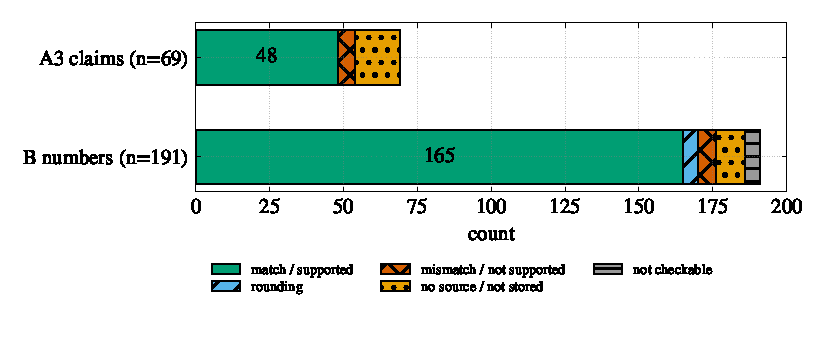
\includegraphics[width=0.78\textwidth]{fig_counts.pdf}
\end{center}

\textbf{Decisions for the author.}
\begin{enumerate}\itemsep0pt
\item L459: the $\pm0.024$ uncertainty is in \texttt{schroeder2014} (p.~4), not \texttt{schroeder2015}; the
  $\pm6.5$\,\% in BR is in neither paper. This settles the open point at L460.
\item L735: \texttt{kaszeta2000} measured a \emph{momentum} diffusivity ratio; the band 1.5--4 cannot be set against
  a heat diffusivity ratio.
\item L189 and L448: the cited papers do not state what is attributed to them.
\item L577--580: intermittency values (15.7, within 0.03, 0.17) do not reproduce from the current detector output.
\item L581: periodic share 0.05--0.08 does not match the source medians (0.025--0.055 or 0.037--0.077).
\end{enumerate}

\textbf{Known states, reported as such and not as findings.} Six \texttt{\%\% OPEN:} markers are present (L178,
L340, L399, L460, L514, L761; Table~\ref{tab:open}). The 20M LES is pending in the coolant budget, the 3D overview
and $\Pr_t$. The jet-region $\Pr_t$ value was removed on purpose and was not checked.

\section*{Method and scope}

The Stage~2.5 INTEGRITY (pre-review) contract of the \texttt{academic-pipeline} skill was followed as the checking
discipline: populations declared, denominators given, unknown states kept visible, a verdict per item. No other
pipeline stage was run. No content was sent to an external model. Web requests were Crossref DOI look-ups only
(bibliographic metadata, no project content).

\begin{center}
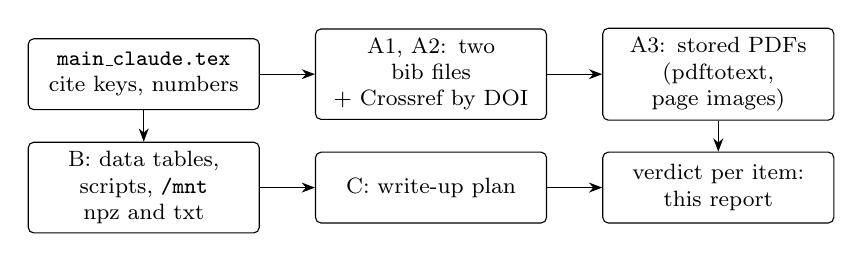
\begin{tikzpicture}[node distance=4mm and 7mm, box/.style={draw,rounded corners=2pt,align=center,font=\footnotesize,minimum height=9mm,text width=27mm}, >=Stealth]
\node[box] (tex) {\texttt{main\_claude.tex}\\cite keys, numbers};
\node[box,right=of tex] (bib) {A1, A2: two bib files\\+ Crossref by DOI};
\node[box,right=of bib] (pdf) {A3: stored PDFs\\(pdftotext, page images)};
\node[box,below=of tex] (dat) {B: data tables, scripts, \texttt{/mnt} npz and txt};
\node[box,right=of dat] (plan) {C: write-up plan};
\node[box,right=of plan] (rep) {verdict per item:\\this report};
\draw[->] (tex) -- (bib); \draw[->] (bib) -- (pdf); \draw[->] (tex) -- (dat); \draw[->] (dat) -- (plan);
\draw[->] (pdf) -- (rep); \draw[->] (plan) -- (rep);
\end{tikzpicture}
\end{center}

\begin{itemize}\itemsep0pt
\item \textbf{A populations.} All 53 \verb|\cite| keys outside comment lines. The build reads both
  \texttt{references.bib} and \texttt{references\_claude.bib}; no key is in both. A3: every sentence that
  attributes a finding, number or method to a source (69 statements); full list in Appendix~\ref{app:a3}.
\item \textbf{B population.} Every number in the abstract, Section~4, all captions, Tables~1 and 2, the conclusions and
  the nine preamble macros (191 items; quantities repeated in one sentence grouped as one item; Methods text outside
  Table~1 not included). Full list in Appendix~\ref{app:b}.
\item \textbf{Read-only recomputation.} Three scripts in this folder import the figure modules:
  \texttt{check\_meff\_split.py}, \texttt{check\_eta.py} and \texttt{check\_gamma.py}. A fourth,
  \texttt{run\_noplot.py}, runs \texttt{fig\_prt\_classic\_span.py} with \texttt{savefig} disabled. Nothing was written outside this folder.
\item \textbf{Verdict codes.} A: \vS{} supported (page = PDF page index), \vNS{} not supported, \vSNS{} source not
  stored. B: \vM{} match, \vR{} rounding only, \vMM{} mismatch, \vNSF{} no source found, \vNC{} not checkable (value
  read from a figure, no tabulated source).
\item \textbf{Failure-mode checklist (skill, 7 modes).} Mode~2 (hallucinated citation): not observed; 53/53 keys resolve,
  51 DOIs, 50 confirmed in Crossref, \texttt{kar2026} DOI not registered there. Mode~3 (hallucinated result): not
  observed; the 10 numbers without a source are listed under ``B. Reported numbers'' below. Modes 1, 4--7 concern
  implementation and framing and were outside the scope set for this check: not assessed.
\end{itemize}

\section*{Findings, ordered by severity}

Severity: \textbf{high} = statement contradicts its source or a claim rests on a misattribution;
\textbf{medium} = number or range differs beyond rounding, or a quoted value has no source; \textbf{low} = rounding,
completeness of metadata, or wording of a bound.

\subsection*{A. Citations}
{\footnotesize
\begin{longtable}{@{}P{9mm} P{9mm} P{42mm} P{49mm} P{49mm}@{}}
\toprule
Sev. & Line & Quoted text & Source says & Proposed correction \\ \midrule\endhead
high & 734--735 & ``$\alpha_y/\alpha_z$ \dots\ 3.2 \dots\ inside the band of 1.5--4 measured by Kaszeta and Simon''
 & \texttt{kaszeta2000} measures eddy diffusivity of \emph{momentum}; ratio $\epsilon_{M,z}/\epsilon_{M,y}$ 1.5--4.0
   near the jet core, 1.5--2.5 over most of the region (p.~5). No heat diffusivity is measured.
 & Compare the band with the momentum ratio $\nu_y/\nu_z$ (0.7--1.1 in the reference, which then lies below the
   band), or drop the comparison of $\alpha_y/\alpha_z$ with this source. \\
high & 458--459 & ``uncertainty is $\pm0.024$ in $\eta$ at 95\,\% confidence and up to $\pm6.5$\,\% in
  $\BR$~\cite{schroeder2015}''
 & \texttt{schroeder2014} p.~4: $\delta\eta=\pm0.024$ at DR~1.5, 95\,\%; BR $\pm10$\,\% at $M=0.5$, $\pm2.9$\,\% for
   $M\ge2$. \texttt{schroeder2015} p.~3: $\delta\eta=\pm0.025$; BR $\pm4.5$\,\% at $M=1.5$. $\pm6.5$\,\% not found.
 & Cite \texttt{schroeder2014} for $\pm0.024$; state BR uncertainty $\pm4.5$\,\% at BR~1.5 with
   \texttt{schroeder2015}. Closes OPEN at L460. \\
high & 447--448 & ``RANS passes 4.7\,\% more coolant \dots, an effect of the model~\cite{haydt2018}''
 & \texttt{haydt2018} sets BR in the CFD; it states that the CFD does not capture mixing and over-diffusion in large
   diffusers (p.~10). No coolant-flow comparison.
 & Remove the citation, or recast: RANS is known to mispredict diffuser flow~\cite{haydt2018}. \\
medium & 187--189 & ``\dots\ come from the model and the resolution alone~\cite{saumweber2003}''
 & \texttt{saumweber2003} is an experiment on FST effects for shaped holes; no such statement.
 & Remove \texttt{saumweber2003} from this sentence. \\
low & 457--458 & ``tripped turbulent approach layer of $\Reth$ 630--700''
 & \texttt{schroeder2014} Table~3 (p.~5): $\Reth=670$ at $Tu=0.5$\,\%; no range.
 & ``$\Reth\approx670$''. \\
low & 450--451 & ``$\etab$ changes by 5--10\,\% between blowing ratios of 1.0, 1.5 and 2.0''
 & Supported for $x/D$ 7--15 (Fig.~8b, p.~7; digitised 0.230/0.243/0.218). Read from Fig.~8b at $x/D\approx17.5$:
   BR~1.0 against 1.5 differs by $\sim$15\,\% (figure reading, $\pm0.01$ in $\etab$; interpretation).
 & Add the window: ``over $x/D$ 7--15''. Counted as \vS. \\
\bottomrule
\end{longtable}}

\textbf{Bibliography completeness (A2), low.} 13 entries lack the article or paper number that Crossref holds:
\texttt{clark2024} (V12BT30A019), \texttt{foroutan2014} (011701), \texttt{haydt2017} (091012), \texttt{haydt2018}
(051002), \texttt{ling2016} (021008), \texttt{milani2017} (021006), \texttt{milani2020} (A27), \texttt{oliver2017}
(V05AT12A005), \texttt{sandberg2018} (101008), \texttt{schroeder2014} (V05BT13A036), \texttt{schroeder2015}
(V05BT12A038), \texttt{schroeder2016} (091001), \texttt{schroeder2016b} (021012). Three more trigger bibtex ``empty
pages'': \texttt{nunno2022} (AIAA 2022-1404, number in DOI only), \texttt{rochhausen2015} (no pages, no DOI, URL only),
\texttt{kar2026} (DOI 10.33737/gpps26-tc-005 not found in Crossref, HTTP 404; check after registration).
\texttt{pope2000} has no ISBN. Key and year differ in \texttt{ling2015} (year 2016) and \texttt{milani2020} (JFM 906,
issue 2021); the year fields agree with Crossref, so no change is needed. Unused entries: 8 in
\texttt{references\_claude.bib} (\texttt{tracy2020}, \texttt{haven1997b}, \texttt{muppidi2008}, \texttt{oliver2019},
\texttt{zamiri2020}, \texttt{hoda2000}, \texttt{haydt2018c}, \texttt{cavar2012}); 59 in \texttt{references.bib}, which
\texttt{main.tex} shares; bibtex prints only cited entries. Unresolved keys: none.

\subsection*{B. Reported numbers}
{\footnotesize
\begin{longtable}{@{}P{9mm} P{9mm} P{39mm} P{53mm} P{47mm}@{}}
\toprule
Sev. & Line & Quoted text & Source and value & Proposed correction \\ \midrule\endhead
medium & 577--578 & ``that of the LES rises with it, within 0.03, to 0.94''
 & \texttt{\_gamma\_extract\_v} (policy threshold, $|y/D|\ge2.81$): max $|\gamma_{LES}-\gamma_{193}|=0.145$ at
   $x/D=11.7$; within 0.03 only for $x/D\ge16$. 0.94 matches (0.938, 0.940).
 & ``and that of the LES joins it from $x/D\sim15$, reaching 0.94 at $x/D=20$''. \\
medium & 581 & ``periodic share \dots\ is 0.05--0.08 in the hole, the jet and the film''
 & \texttt{lav\_probes\_c193b.txt} (analysis/coherent\_lav), $\Gamma_\mu$ medians: hole 0.030, jet 0.055, film
   0.025--0.048 ($\sigma$ Lav); 0.045, 0.077, 0.037--0.070 ($\sigma$ 0.036).
 & ``0.03--0.06'' (or 0.04--0.08 with $\sigma=0.036$, naming the choice). \\
medium & 562 & ``shape factor \dots\ within 0.03 of the Blasius value of 2.59''
 & \texttt{bl\_extract/c193b\_b010.npz}: span-mean $H$ 2.61--2.62 for $x/D<-6$; 2.64 at $x/D$ $-6$ to $-4$; 2.67 at
   $-4$ to $-2$.
 & ``within 0.03 of 2.59 for $x/D<-6$, rising to 2.67 just upstream of the hole''. \\
medium & 671 (macro) & \verb|\Lnear| ``the RANS length is 0.45--0.5 of the reference''
 & \texttt{\_meff\_split\_nearfar.compute\_curve}, slabs 4.5--19.5: $L$ ratio 0.429--0.499.
 & \verb|\Lnear| = 0.43--0.50. \\
medium & 580 & ``mean $\gamma$ of the RANS is 0.17''
 & No source found. \texttt{bl\_extract/rans50\_z010\_cells.npz} gives 0.18 (span-binned, $x/D$ $-3$ to 20) or 0.24
   (cell mean). Reference 0.726 over $x/D$ $-3$ to 20 (0.816 over 0 to 20).
 & State the averaging range and recompute both values on it. \\
medium & 416 & ``regional values of the reference move by 0.046 or less''
 & No source found in \texttt{figures/code/data} or \texttt{/mnt/.../asme2027\_figs}.
 & Add the source table or remove the number. \\
low & 577 & ``$\gamma$ \dots\ exceeds 0.8 from $x/D=15.7$''
 & Same source: first above 0.8 at $x/D=15.52$, above 0.8 from 15.58 onward.
 & ``from $x/D=15.6$''. \\
low & 528 & ``RANS turbulent flux is 0.67--0.98 of the reference'' ($z/D=1.0$)
 & \texttt{n7\_series\_c193b\_b010\_rans50.txt}: 0.672--0.992 over 65 stations $x/D$ 4--20; 0.672--0.983 at the five
   stations of \texttt{mean\_features\_table.txt}.
 & ``0.67--0.99''. \\
low & 655 & ``it holds 19 cells, four of them with a ratio of 3 or more''
 & Printed by \texttt{fig\_meff\_maps.py} at run time; not reproduced, since that script also writes data files.
   Line end points 1.36 and 1.41 match.
 & None; confirm from the last run log. \\
low & 697 & ``$\Leff$ is within 7\,\% of the dissipation length''
 & No source found; \texttt{fig\_budget\_lines.py} docstring states ``within 5\,\% in the film''.
 & Confirm the value and its region. \\
low & T1 & cell counts $5.77\times10^6$ \dots\ $1.92\times10^8$; $s=0.30$ (5M)
 & No source found in the files checked; $s$ 0.453, 0.628, 0.796 match \texttt{write\_up/methods/03\_mesh\_resolution.tex}.
 & Add the CGNS count table to \texttt{figures/code/data}. \\
low & 94, 464, 873 & ``29--33\,\% low beyond $x/D=7$''
 & Window means (\texttt{fig\_eta\_x}): RANS 50M 29.1\,\% (7--15), 33.7\,\% (15--20); RANS 5M 27.8, 33.7\,\%. Point-wise
   over $x/D$ 7--20: 22--34\,\%. \vR.
 & ``29--34\,\% low over $x/D$ 7--20 (window means)''. \\
low & macro & \verb|\muNearLow| 0.55
 & 0.555 at $x/D=19.5$ (slab range 0.555--0.671). \vR.
 & 0.56, or keep 0.55 and state truncation. \\
low & 580 & reference plane-mean $\gamma$ 0.72
 & 0.726 ($x/D$ $-3$ to 20). \vR.
 & 0.73, with the range stated. \\
low & 94, 396, 463, 871 & ``within 0.008''
 & Bound holds: window means differ by at most 0.006 (20M LES), point-wise by at most 0.007. \vM.
 & Optional: ``within 0.007''. \\
\bottomrule
\end{longtable}}

\textbf{Interpretation, low.} L737: ``mainly through the $\Pr_t$ setting''. In \texttt{prt\_data\_tables.txt} the
$\Pr_t$-setting term is $-0.72$ at $x/D=10$ and the anisotropy term $-0.80$; at $x/D=20$ the $\Pr_t$ term ($-0.47$)
is the largest negative term. The statement holds at $x/D=20$ only.

\textbf{Two sources for one value.} L725 0.23 ($x/D$ 3--10) matches the volume sum over the mesh bins printed by
\texttt{fig\_prt\_classic\_span.py} (0.226); \texttt{prt\_volume\_se.txt} gives $0.2246\pm0.0048$, which rounds to
0.22. Counted as \vM; one source should be named in the data folder.

\textbf{Internal consistency.} Each repeated quantity carries one value across abstract, body, captions, tables and
conclusions: $\etab$ agreement (0.008 for all rungs; 0.006 for the 20M LES), RANS deficit 29--33\,\%, crossing at
$x/D\sim4.5$, near-wall ratio \verb|\muNearLow|--\verb|\muNearHigh| (= 33--45\,\% low at L691), LES within 10\,\%,
CRVP 1.2--1.5, plume 0.75, $\Pr_t$ 0.23--0.45, Table~2 values quoted in Section~4.3. Ranges in the text agree with
Table~2 (36--48\,\%, 34 against 44\,\%, 72, 76, 97, 63\,\%). Line colours and styles named in the text match the
scripts (\texttt{fig\_aposteriori.py}, \texttt{fig\_meff\_split\_film.py}, \texttt{fig\_coolant\_budget.py}); panel
references match the current previews (\texttt{50\_fig\_coolant\_budget\_2x2\_full}, \texttt{56\_fig\_meff\_split\_les},
\texttt{55\_fig\_aposteriori\_les}). The two Table~2 rows ``near the hole'', noted as absent from the data table in
OPEN L761, match \texttt{starccm/\dots\_prtlocal/compare/prtlocal\_eta\_windows\_x20.txt} (34.1\,\%, 0.4687, 0.0080,
0.157; 95.9\,\%, 0.4747, 0.0083, 0.200).

\subsection*{C. Plan mirror}
One numerical difference was found between \texttt{planning/writeup\_plan.tex} and the manuscript. Plan L353--354 gives
$\Pr_t$ at $z^+$ 14: $0.95\pm0.15$, 20: $0.87\pm0.10$, 27: $0.89\pm0.10$; manuscript L714 gives
``$0.9\pm0.1$ for $z^+$ of 15--27''. The script output gives $0.98\pm0.18$ at $z^+=13.4$ and $0.89\pm0.10$ at 26.8
(span, far film). Plan-only numbers with no counterpart in the manuscript (no conflict): swap ranges over $x/D$ 4--20
(velocity 1.2--3.2, coolant 1.4--2.8), layer-mean split terms ($-0.54$; $+0.02$, $-0.27$, $-0.70$, $+0.41$), mid-pitch
$\eta$ 0.008--0.012 for the $\Pr_t$ runs, $k^{1/2}$ 1.10--1.16 and length 0.77--0.85 above $z_x$. No claim differs.

\begin{table}[h]
\centering\footnotesize
\caption{\texttt{\%\% OPEN:} markers in \texttt{main\_claude.tex} (known states).}\label{tab:open}
\begin{tabular}{@{}l P{140mm}@{}}
\toprule
Line & Content \\ \midrule
178 & RANS error in $\etab$ from the literature not yet stated. \\
340 & Time-integration scheme of 3DNS not stated. \\
399 & Fig.~resolution panel (b) pooled over $x/D$ 2.36--25; 5M curve and wall units at the plate pending. \\
460 & Uncertainty source \texttt{schroeder2015} or \texttt{2014}: settled here, \texttt{schroeder2014} p.~4. \\
514 & 20M LES to be added to the coolant budget, 3D overview and $\Pr_t$. \\
761 & Three a posteriori runs unfinished; shares of the last two rows from window means; near-hole rows not in the data table. \\
\bottomrule
\end{tabular}
\end{table}

\clearpage
\section*{Re-run, 28 November 2026}

\textbf{Status: PASS WITH FINDINGS.} One mismatch and two rounding differences remain among the new or changed
items. All twelve findings of the first check are resolved as written.

\textbf{Population.} Every number and every source-attributed claim in \texttt{main\_claude.tex} that is new or
changed since commit 47891ec (\texttt{git diff 47891ec}, read-only; HEAD 3865fed). Sources:
\texttt{coolant\_budget\_les\_table.txt}, \texttt{les\_counterparts\_table.txt}, \texttt{meff\_les\_table.txt},
\texttt{aposteriori\_table.txt} (all in \texttt{figures/code/data}), \texttt{n8\_lsq/prt\_classic\_c20bw\_b006\_jk.json},
the stored Schroeder PDFs and the outputs of the first check. Line numbers refer to the current file.

\begin{center}
\begin{tabular}{@{}l r r r r r r@{}}
\toprule
Population (re-run) & checked & match & rounding & mismatch & no source & not checkable \\
\midrule
A attributed claims, new or changed & 6 & 6 & -- & 0 & 0 & 0 \\
B numbers, new or changed & 70 & 67 & 2 & 1 & 0 & 0 \\
First-check findings (6 NS, 6 MM) & 12 & 12 resolved & -- & 0 & -- & -- \\
\bottomrule
\end{tabular}
\end{center}

\subsection*{Re-run findings}
{\footnotesize
\begin{longtable}{@{}P{9mm} P{9mm} P{42mm} P{55mm} P{44mm}@{}}
\toprule
Sev. & Line & Quoted text & Source and value & Proposed correction \\ \midrule\endhead
low & 509 & ``and the LES cores within $0.01D$ (not shown)''
 & \texttt{les\_counterparts\_table.txt} a: mean of (LES $-$ 193M) core height over $x/D$ 6--20 is $+0.010D$;
   per station $-0.002$, $+0.015$, $+0.027$, $-0.041D$ at $x/D$ 6, 10, 15, 20. \vMM{} (mean quoted as a bound).
 & ``and the LES cores $0.01D$ above on average (within $0.04D$ at every station)''. Plan L252 carries the same
   wording. \\
low & 599--600 & ``the mean $\gamma$ of the RANS is 0.17, against 0.73 for both the reference and the LES''
 & Two grids. 0.04\,$D$ grid (\texttt{fig\_wall\_state} route): RANS 0.167, reference 0.724, LES 0.726. Native
   0.02\,$D$ detector grid: reference 0.7256, LES 0.7278; RANS 0.175 by layer interpolation (first check), not
   reproduced by the other route (variants 0.167--0.180). \vM, route note.
 & ``0.17'' is safe for 0.167 and is a truncation of 0.175 (0.18 by rounding). Same-grid pair: ``0.17 against 0.72''
   (0.04\,$D$), or ``0.17--0.18 against 0.73''. \\
low & 553 & ``the RANS coolant field alone by 2.7''
 & \texttt{swap\_lateral\_table.txt}: 2.65 at $x/D=10$. \vR. & None needed; 2.65 rounds to 2.7. \\
low & 601--602 & ``periodic share of 0.03--0.06''
 & \texttt{lav\_probes\_c193b.txt}, $\sigma$ of Lav: 0.025--0.055 (hole 0.030, jet 0.055, film 0.025--0.048). \vR.
 & None needed. \\
\bottomrule
\end{longtable}}

\textbf{Still without a source (unchanged since 47891ec, outside the re-run population).} L676 ``19 cells, four of them
with a ratio of 3 or more''. The 0.046 (L418), the 7\,\% (L724) and the Table~1 cell counts (L310) are now under
\texttt{\%\% OPEN:} markers.

\subsection*{Point 1: 20M LES numbers}
All match their sources. Coolant budget (\texttt{coolant\_budget\_les\_table.txt}): turbulent flux above mean-flow
flux from $x/D=4.0$; turbulent 1.07--1.19 of the reference at the six stations; mean-flow 0.92, 0.88 ($x/D$ 4, 5),
0.39 ($x/D$ 10), $-0.90$ against $+0.85$ ($x/D$ 20); SGS part $\le0.05$\,g\,s$^{-1}$\,m$^{-1}$; LES total below the
reference at every station; lateral inward mean 0.85 ($x/D$ 5), outward turbulent 0.90--1.03, lowest at $x/D=10$;
CRVP circulation 0.887--0.986 (0.89--0.99), WV 0.701--1.225 (0.70--1.23); 0.0905 at $x/D=4$ (0.091).
Fixed-height planes (\texttt{les\_counterparts\_table.txt} b): $z/D=1.0$ 0.95--1.17, 0.25 0.91--1.50, 0.5 1.04--1.48,
LES turbulent flux positive at all 65 stations. Upwash 0.69--1.09 (lowest at $x/D$ 20), inward velocity 0.87--1.08,
half-width 1.030, centroid 1.012. Eddy viscosity (f, g): $k^{1/2}$ 1.008 and 1.011, $\cos\theta$ ratio 0.959 and
0.984, length 1.114 and 1.177; cross-plane median $k$ 1.05--1.11, median length 1.14--1.26; layer means 1.067 and
1.143 (\texttt{meff\_les\_table.txt}). $\Pr_t$ (json, total = resolved + SGS): $0.2142\pm0.0068$, $0.4595\pm0.0218$;
reference 0.226 and 0.450, so ``within one standard error'' and ``0.01 below'' hold. Diffusivities (h):
$\alpha_y/\alpha_z$ 1.88 and 1.66, intervals overlapping at $x/D=10$ ([2.34, 4.70] against [1.58, 3.47]);
$\nu_y/\nu_z$ 0.98, 0.75; lateral heat diffusivity 1.102, 1.059. Table~2 LES row: 0.365, 0.028, 0.202; the 91\,\%
cell is $1-(0.2259-0.2199)/(0.2259-0.1565)=91.4$\,\% from the window means weighted 8:5, as footnote $b$ defines.

\subsection*{Point 2: first-check findings}
\begin{itemize}\itemsep0pt
\item L763 Kaszeta: ``\dots\ below the 1.5--4 that Kaszeta and Simon measured for the same ratio near the jet core at
  $x/D=2.5$ behind cylindrical holes.'' \vS{} (p.~5, Fig.~8; p.~1--2: 35°, $I=1$, DR~1, $Tu\approx12$\,\%).
\item L462--463: ``$\Reth\approx670$; \dots\ $\pm0.024$ \dots\ \cite{schroeder2014} and $\pm4.5$\,\% in $\BR$ at a
  blowing ratio of 1.5~\cite{schroeder2015}.'' \vS{} (2014 p.~4, p.~5; 2015 p.~3).
\item L451--452: ``RANS has been found not to capture the mixing in large diffusers~\cite{haydt2018}.'' \vS{} (p.~10).
\item L189: \texttt{saumweber2003} removed. Resolved.
\item L597--599: ``exceeds 0.8 from $x/D=15.5$ \dots\ differs from it by up to 0.145, at $x/D=11.7$, lies within 0.03 of
  it from $x/D=16$ and reaches 0.94''. \vM.
\item L582: ``within 0.03 of the Blasius value of 2.59 for $x/D<-6$ and rises to 2.67''. \vM. L543: 0.67--0.99 \vM.
  \verb|\Lnear| 0.43--0.50 \vM. L601: 0.03--0.06 \vR.
\item L739--742: ten flow-through times; ``about eleven times the record'' ($(0.332/0.1)^2=11.0$, median SE of the
  strip); not resolved below $z^+\approx11$ (flagged to 10.7); ``$z^+$ of 13--30 ($z/D$ 0.10--0.22) it is 0.9--1.0
  ($\pm$0.10--0.18)'': $0.98\pm0.18$ (13.4), $0.89\pm0.10$ (26.8), $0.88\pm0.10$ (29.5). \vM.
\item L505--507 circulation: smoothing $\sigma=(2,3,3)$ cells of $0.05D$ = 0.10--0.15$D$; reference 0.0960, 0.0658,
  0.0408 in both analyses; RANS/193M 1.142, 1.217, 1.138 smoothed and 1.47 on the fine planes. Conclusion L907
  ``1.1--1.5 times'' covers 1.14--1.47. \vM.
\end{itemize}

\subsection*{Point 3: verification-pass statements}
L474 ``in $\Tu$ (0.5 against 5.5\,\%), in $\ReD$ (4960 against 2408) and in Mach number (0.03 against 0.25)'': the
first value of each pair is the experiment, the second the simulations. Experiment: $Tu=0.5$\,\%
(\texttt{schroeder2014} p.~5); $U_\infty=10$\,m\,s$^{-1}$, 295\,K, $D=7.75$\,mm (\texttt{schroeder2015} p.~2), which
gives $\ReD\approx5000$ and Mach 0.029. Simulations: L285--288 (Mach 0.25, $Tu$ 5.5\,\%, $\ReD=2408$). \vM. The
``ten flow-through times'' and ``about eleven times the record'' are confirmed under Point 2.

\subsection*{Point 4: internal consistency and plan}
Each quantity carries one value wherever it appears: LES circulation 0.89--0.99 (L510, L909; plan L252, L443); LES
$\Pr_t$ 0.21--0.46 (L752--753, L914; plan L365, L446); LES eddy viscosity within about 10\,\% and 1.14 (L711--713,
L884, L913; plan L347--349, L422, L445); $\etab$ within 0.006 (L864, L884, L886, L921; plan L416, L421, L450); lateral
profile 0.029 against 0.043 (L865--866, L886, L921; plan L417, L423); RANS deficit 29--34\,\% (L95, L466, L902; plan
L111, L242, L439); wall-layer $\Pr_t$ (L741--742, L879; plan L362, L425). The plan repeats the L509 core wording
(finding above). Plan-only detail with no conflict: LES $\Pr_t$ SGS part under 0.001 (json: 0.0003 and 0.0005).

\clearpage
\appendix
\section{Population A3: attributed claims}\label{app:a3}
{\footnotesize
\begin{longtable}{@{}r P{11mm} P{36mm} P{70mm} P{12mm} P{18mm}@{}}
\toprule
\# & Line & Key(s) & Claim & Verdict & Page \\ \midrule\endhead
1 & 171 & bogard2006 & bleed coolant costs cycle efficiency & \vS & 2 \\
2 & 174 & gritsch1998, thole1998, saumweber2003 & shaped holes higher $\eta$ than cylindrical at high BR & \vS & 1, 1, 1 \\
3 & 176 & milani2017, milani2020 & design relies on RANS & \vS & 1 (2017) \\
4 & 181--184 & schroeder2014 & 30°, 7°, $6D$, AR 2.5, pitch $6D$; peak near BR 1.5 at DR 1.2, 1.5 & \vS & 1 \\
5 & 185--186 & schroeder2016, 2016b, haydt2017, haydt2018 & database: flow, thermal field, FST, offset, AR & \vS & 1 \\
6 & 187--188 & oliver2017, nunno2022, bin2024 & simulations on flat plate, ZPG & \vS & 3; 4; 2 \\
7 & 189 & saumweber2003 & differences from model and resolution alone & \vNS & -- \\
8 & 191--192 & acharya2001, harrison2008, foroutan2014, stratton2019 & lateral spread low, centreline high & \vS & 6; 2--3; 1, 6; 1 \\
9 & 192--193 & haydt2017 & steady RANS misses level and offset trend & \vS & 1 \\
10 & 193--194 & laroche2023 & SST centreline $\sim$25\,\% high beyond $x/D=10$ & \vS & 10 \\
11 & 207 & azzi2002, laroche2023 & CRVP too strong (Azzi: size exaggerated) & \vS & 12; 11 \\
12 & 207--209 & stratton2019, coletti2013 & SST over, $k$--$\varepsilon$ under & \vS & 6; 1 \\
13 & 209--210 & kaszeta2000, kohli2005, coletti2013 & diffusivities non-uniform, anisotropic & \vS & 1, 5; 5; 11 \\
14 & 210--211 & ling2016, stratton2019 & Boussinesq fails in hole, at wall, lee side & \vS & 1; 1 \\
15 & 211--212 & stratton2019 & $\Pr_t$ in jet below setting & \vS & 10 \\
16 & 212--215 & azzi2002, lakehal2002, liu2008, liu2011, ling2015, milani2017/2020 & corrections per assumption & \vS & 1 each \\
17 & 217--219 & oliver2017 & peak turbulent flux $\sim$15\,\% of mean, $x/d\le5$ & \vS & 10 \\
18 & 219--220 & coletti2013 & turbulent dominates beyond $\sim3D$ & \vS & 4 \\
19 & 220--221 & schroeder2016b & BR 3 jet top: mean-flow transport & \vS & 5 \\
20 & 222--224 & foroutan2014 & RANS wall-normal flux close to DES; lift-off missed at 1.5 & \vS & 8 \\
21 & 224--225 & milani2020 & isotropic diffusion over-spreads at fixed LES velocity & \vS & 20 \\
22 & 230--231 & fric1994 & HV, wake, shear-layer vortices & \vS & 2 \\
23 & 232 & tyagi2003 & hairpin packets cause hot spots & \vS & 1 \\
24 & 232--233 & fawcett2013 & coherent structures only at large velocity difference & \vSNS & -- \\
25 & 238--239 & clark2024 & transitional $3\times10^5<Re_x<10^6$; small cores & \vS & 1 \\
26 & 240 & kar2026 & tripping depends on size, spacing, position & \vS & 1 \\
27 & 241 & goldstein1982 & holes trip a laminar layer & \vS & 1 \\
28 & 241 & langtry2009 & transition model holds layer laminar & \vS & 1--2 \\
29 & 243--244 & oliver2017, nunno2022 & iLES at BR 2, laminar approach; $\Delta\eta\sim0.05$ from resolution & \vS & 2, 3, 6; 1, 3, 4 \\
30 & 244--245 & bin2024 & DNS on $78\times10^6$ cells, turbulent inflow & \vS & 2, 4 \\
31 & 279 & schroeder2014 & baseline hole, $D=7.75$\,mm, 30°, pitch $6D$ & \vS & 1, 4 \\
32 & 329 & menter1994 & SST model & \vSNS & -- \\
33 & 329 & langtry2009 & $\gamma$--$\Reth$ model & \vS & 1 \\
34 & 332 & wheeler2016 & 3DNS solver & \vSNS & -- \\
35 & 333 & tam1993 & DRP stencil & \vSNS & -- \\
36 & 334 & nicoud1999 & WALE model & \vSNS & -- \\
37 & 386 & pope2000 & $\kappa_{\max}\eta_K\ge1.5$ & \vSNS & -- \\
38 & 448 & haydt2018 & RANS excess coolant a model effect & \vNS & 10 \\
39 & 450--451 & schroeder2014 & $\etab$ changes 5--10\,\% over BR 1.0--2.0 & \vS & 7 \\
40 & 456--458 & schroeder2014 & $Tu$ 0.5\,\%, Mach 0.03, $\ReD\approx4960$, tripped layer & \vS & 3, 5 (Ma, $\ReD$ derived) \\
41 & 458 & schroeder2014 & $\Reth$ 630--700 & \vNS & 5 \\
42 & 458--459 & schroeder2015 & $\pm0.024$ in $\eta$, 95\,\% & \vNS & 3 \\
43 & 459 & schroeder2015 & $\pm6.5$\,\% in BR & \vNS & 3 \\
44 & 493 & haven1997, fric1994, haydt2018 & hole vorticity leaves as streamwise vortices & \vS & haydt 2 \\
45 & 494 & haven1997 & anti-kidney pair & \vSNS & -- \\
46 & 502--503 & laroche2023, stratton2019 & too-strong CRVP from contours & \vS & 11; 6 \\
47 & 554--555 & stratton2019 & weaker $k$--$\varepsilon$ pair, no more spreading & \vS & 6 \\
48 & 555--556 & acharya2001, harrison2008 & RSM did not widen film & \vS & 7; 1 \\
49 & 565 & otsu1979 & threshold method & \vSNS & -- \\
50 & 566--567 & dellacasagrande2023 & Otsu on spanwise stress & \vS & 3 \\
51 & 580 & lav2019 & triple decomposition & \vS & 3 \\
52 & 582 & fawcett2013 & broadband mixing at VR near 1 & \vSNS & -- \\
53 & 608 & wu2018, mcconkey2022 & point-wise optimal eddy viscosity & \vSNS & -- \\
54 & 610 & kohli2005 & classic $\Pr_t$ form & \vS & 3 \\
55 & 639 & schmitt2007 & stress--strain angle test & \vSNS & -- \\
56 & 651 & stratton2019 & masked comparison & \vS & 8 \\
57 & 682--683 & stratton2019 & SST below LES least-squares value; near-wall misalignment & \vS & 1, 11 \\
58 & 684 & sandberg2018 & poor near-wall alignment, slot & \vS & 5 \\
59 & 704 & kays1994 & 0.85--0.9 in log layers & \vSNS & -- \\
60 & 705 & schlichting2017 & free-shear $\sim$0.5 & \vSNS & -- \\
61 & 726--727 & kohli2005 & $\Pr_t\sim2$ low FST, $\sim1$ high FST & \vS & 7 \\
62 & 727--728 & ling2015, liu2008, liu2011, stratton2019 & low, varying $\Pr_t$ & \vS & 1; 1; 1; 10 \\
63 & 729 & rochhausen2015 & $\Pr_t$ 0.9 under-spreads by $\sim$20\,\% & \vSNS & -- \\
64 & 734--735 & kaszeta2000 & heat diffusivity ratio band 1.5--4 & \vNS & 5 \\
65 & 745--747 & liu2008/2011, lakehal2002, milani2017/2020, azzi2002, spalart2000 & remedies per input & \vS & 1; 1; 1; 1; 2 \\
66 & 747--748 & langtry2009 & no film-cooling trip & \vS & absence \\
67 & 824 & spalart2000 & QCR stress & \vS & 2 \\
68 & 845--846 & fawcett2013 & coherent structures at other BR & \vSNS & -- \\
69 & 789 & schroeder2014 & experiment row of Table~2 (database file id727) & \vS & data \\
\bottomrule
\end{longtable}}
Totals: \vS{} 48, \vNS{} 6, \vSNS{} 15.

\section{Population B: reported numbers}\label{app:b}
Values checked as listed. Sources: D = \texttt{figures/code/data/}; W = \texttt{/mnt/.../asme2027\_figs/wall\_balance/};
G = recomputation in \texttt{planning/integrity\_check/}.
{\footnotesize
\begin{longtable}{@{}P{15mm} P{58mm} P{75mm} P{10mm}@{}}
\toprule
Line & Number(s) & Source & Verdict \\ \midrule\endhead
\multicolumn{4}{@{}l}{\textit{Preamble macros (9)}}\\
52--59 & xEVstart 4; fEVmin 20; zxStart 0.59; zxEnd 0.94 & D near\_wall\_boundary\_zx.txt (0.5914, 0.9420); FMIN 0.2 & 4\,\vM \\
55 & muNearLow 0.55 & G check\_meff\_split: 0.555 & \vR \\
56 & muNearHigh 0.67 & G: 0.671 & \vM \\
57 & Lnear 0.45--0.5 & G: 0.429--0.499 & \vMM \\
58--59 & cosNearStart 2.5; cosNearEnd 1.7 & G: 2.46, 1.73 & 2\,\vM \\
\multicolumn{4}{@{}l}{\textit{Abstract (7)}}\\
92 & DR, BR 1.5 & Table~1 BR 1.498--1.592 & \vM \\
93 & 20M to 193M & Table~1 & \vM \\
94 & within 0.008 & fig\_eta\_x windows max 0.006; G point-wise 0.007 & \vM \\
94 & 29--33\,\% & windows 29.1--33.7\,\% & \vR \\
95 & $x/D\sim4.5$ & W n7\_surface\dots zxpt: first at 4.50 & \vM \\
97--98 & LES within 10\,\% & D meff\_les\_table: 0.977--1.091 & \vM \\
98 & $\Pr_t$ 0.23--0.45 & fig\_prt\_classic\_span: 0.226, 0.450 & \vM \\
\multicolumn{4}{@{}l}{\textit{Table 1 (25)}}\\
317--322 & $s$ 0.453, 0.628, 0.796, 1 & write\_up/methods/03\_mesh\_resolution.tex & 4\,\vM \\
317 & $s$ 0.30 (5M) & none found & \vNSF \\
317--322 & cells (5 values) & none found & 5\,\vNSF \\
317--322 & filter 0.03, 0.05, 0.03, 0.03 & write\_up/methods/02\_simulation\_ladder.tex & 4\,\vM \\
317--322 & BR 1.591, 1.498, 1.592, 1.516, 1.526, 1.521 & hole\_discharge/results/summary.txt & 6\,\vM \\
317--322 & 6\,FT (4), 10\,FT & ladder text, b010 & 5\,\vM \\
\multicolumn{4}{@{}l}{\textit{Table 2 (54)}}\\
775--789 & 11 recovered shares; 14 centreline; 14 mid-pitch; 14 $\etab$; caption BR 1.416 & D aposteriori\_table.txt; starccm prt\_eta\_windows, prtlocal\_eta\_windows\_x20 & 54\,\vM \\
\multicolumn{4}{@{}l}{\textit{Section 4 body (79)}}\\
415--416 & 6, 10\,FT & text & \vM \\
416 & 0.046 & none found & \vNSF \\
439 & 0.141, 0.096 & D mean\_features (fine planes 0.1414, 0.0960) & \vM \\
446 & about twice near $s/D=-2$ & sections\_*.txt rev 0.159 / 0.094 (1.7); 20M--100M 1.8--2.2 & \vM \\
447 & 4.7\,\% & summary.txt 1.5919/1.5208 & \vM \\
449 & 1.2\,\%, St 0.27 & bubble3d\_c193b.txt 0.0185/1.5273, 0.273 & \vM \\
457 & $|y/D|=2.91$ & fig\_eta\_x & \vM \\
462--463 & windows, 0.008, a third & fig\_eta\_x log & \vM \\
464 & $x/D\sim4$ & figure only & \vNC \\
464 & 29--33\,\% & as abstract & \vR \\
469 & $\sim$0.035 from $x/D=2$ & aposteriori (0.037, 0.033, 0.033, 0.035) & \vM \\
470 & near zero to $x/D=9$ & figure only & \vNC \\
494 & $x/D\sim3$ & figure only & \vNC \\
498 & 0.2 of peak & mean\_features header & \vM \\
499 & 1.5 at 4, 1.2 at 20 & fine planes 1.47, 1.16 & \vM \\
500 & half peak; $\sim0.1D$ & fine planes 0.08--0.13 & \vM \\
501 & WV 4--15; RANS lost from 5 & mean\_features WV rows & \vM \\
520 & $\Pr_t=0.9$ & RANS setting & \vM \\
525--526 & $x/D\sim4.5$ & W zxpt & \vM \\
527 & 0.37--0.61 & W zxpt 0.374--0.613 & \vM \\
527 & 1.9--5.9 & W zxpt 1.871--5.939 & \vM \\
528 & 0.67--0.98 & W n7\_series 0.672--0.992 & \vMM \\
528--529 & towards wall at 0.25; ordering at 0.25, 0.5, 1.0 & W n7\_series & \vM \\
530 & 5\,\%, 1.2\,\% & W n7\_summary 4.95\,\%, 1.16\,\% & \vM \\
536 & 2.7, 2.65, 5.2 & D swap\_lateral 2.71, 2.65, 5.23 & \vM \\
545 & every station; 1.86 & W n7\_swap\_lateral 1.30--1.86 & \vM \\
546 & 0.29 at 4; 15--20 & W 0.288; reaches 1 at 17.5 & \vM \\
552 & 1.14--1.66 & mean\_features W/U centre & \vM \\
553 & 1.75--1.93 & mean\_features V/U & \vM \\
557 & 0.75 & mean\_features 0.750 & \vM \\
557 & within 12\,\% & mean\_features 1.006--1.119 & \vM \\
562 & within 0.03 of 2.59 & bl\_extract 2.61--2.67 & \vMM \\
563--564 & $z/D$ 0.1, $2D/U$, $1D/U$ & \_gamma\_extract\_v & \vM \\
572 & $x/D\sim8$ & bl\_extract mid-pitch & \vM \\
576 & $x/D\sim10$ & figure only & \vNC \\
577 & 0.8 from 15.7 & G 15.52--15.58 & \vMM \\
578 & within 0.03 & G max 0.145 & \vMM \\
578 & 0.94 & G 0.938, 0.940 & \vM \\
579 & 0.02 & bl\_extract rans50\_z010 0.021 & \vM \\
580 & 0.17 & G 0.18--0.24 & \vNSF \\
580 & 0.72 & G 0.726 & \vR \\
581 & 0.05--0.08 & lav\_probes\_c193b.txt & \vMM \\
621, 651 & $z/D\ge0.3$; 0.05 & scripts & 2\,\vM \\
654 & 4--4.25; 1.36--1.41 & fig\_meff\_maps JET\_MASK & \vM \\
655 & 19 cells, four & not reproduced & \vNSF \\
656, 660 & 4 to 20 & macros & \vM \\
662 & $0.02D$; 3.5 & review/45\_zx\_crosscheck.txt 0.018 & \vM \\
663--664 & $\pm0.02D$, $\pm0.04D$ & 45\_zx\_crosscheck (0.047, 0.049, 0.087 ranges) & \vM \\
669 & slabs $1D$ & script & \vM \\
678 & 1.06 & G 1.056 & \vM \\
679 & $\sim$0.8 & G 0.800 & \vM \\
680 & 1.23--1.45 & G 1.232--1.452 & \vM \\
681 & 32--56\,\% & G 0.320--0.557 & \vM \\
688--689 & $0.1D$; 0.03 & D meff\_les\_table (0.027) & \vM \\
690 & 1.07; 10\,\% & D 1.067; 0.977--1.091 & \vM \\
691 & 33--45\,\% & G 32.9--44.5 & \vM \\
692--693 & 1.14; 1.23; 1.06 & D 1.143, 1.233, 1.056 & \vM \\
697 & 7\,\% & none found & \vNSF \\
706--710 & $0.1D$; 0.05; twice SE & fig\_prt\_classic\_span & \vM \\
712 & 46\,\% & G 0.460 & \vM \\
713 & $z^+\sim10$ & G flagged to 10.7 & \vM \\
714--715 & $0.9\pm0.1$, $z^+$ 15--27, $z/D$ 0.11--0.2 & G $0.98\pm0.18$ (13.4), $0.89\pm0.10$ (26.8) & \vM \\
716 & 0.45, twice & G 0.450 & \vM \\
725 & 0.23; 0.45 & G 0.226; 0.450 & \vM \\
734--735 & 3.2; 0.7--1.1 & prt\_data\_tables 3.16; 1.07, 0.71 & \vM \\
737 & 0.5--0.6 & prt\_data\_tables 0.54, 0.63 & \vM \\
755--758 & windows; 2\,\% & aposteriori BR 1.5613--1.5945 & \vM \\
805 & within 0.04 & 0.035 & \vM \\
807--809 & 36--48\,\%; 34, 44\,\% & Table~2 sources & \vM \\
815--819 & 76\,\%; 0.03; 12\,\% & aposteriori & \vM \\
825--827 & 72\,\%; 97\,\% & Table~2 & \vM \\
828 & $x/D\sim7$ & figure only & \vNC \\
830 & 11\,\% & 1.4161/1.5925 & \vM \\
835--837 & 0.006; 0.029, 0.043; 0.02--0.04 & aposteriori & \vM \\
844 & BR, DR 1.5, VR 1.0, $Tu$ 5.5\,\% & Methods, Table~1 & \vM \\
848 & 0.3--0.5; less than half & Table~2 & \vM \\
850 & $z^+$ 15--27, $\sim$0.9 & as 714 & \vM \\
855 & 0.006; 10\,\% & as 835, 690 & \vM \\
\multicolumn{4}{@{}l}{\textit{Captions (5)}}\\
423--424 & $Q$ 0.005; $x/D$ 2, 4, 10 & fig\_overview\_3d CFG & \vM \\
407 & $\deta=2$ & fig\_resolution & \vM \\
485 & $|y|=0.5D$ & n7\_swap\_lateral & \vM \\
508 & $z/D=0.1$ & spots & \vM \\
799 & $x/D$ 15--20 & fig\_aposteriori & \vM \\
\multicolumn{4}{@{}l}{\textit{Conclusions (12)}}\\
866--869 & DR, BR 1.5; 5--193M; 10\,FT & Table~1 & 3\,\vM \\
871 & 0.008 & as abstract & \vM \\
873 & 29--33\,\% & as abstract & \vR \\
875 & $x/D\sim4.5$ & W zxpt & \vM \\
877--878 & 0.75; 1.2--1.5 & mean\_features & 2\,\vM \\
883 & $\sim$10\,\%; 1.14 & meff\_les\_table & \vM \\
884 & 0.23--0.45; 0.9 & as 725 & \vM \\
885 & $\Pr_t=0.4$ & Table~2 & \vM \\
888--889 & 0.006; 0.029; 0.04 & aposteriori & \vM \\
\bottomrule
\end{longtable}}
Totals (191): \vM{} 165, \vR{} 5, \vMM{} 6, \vNSF{} 10, \vNC{} 5. Body rows that bundle several values in one
sentence count as one item.

\end{document}
